\documentclass[12pt,letterpaper]{article}
\usepackage{graphicx}
\usepackage{xfrac}
\usepackage{mcode}
\usepackage{subcaption}
\captionsetup{compatibility=false}

\begin{document}

\title{HW5 - Music Genre Identification}
\author{Beichen Su}

\maketitle

\begin{abstract}
Using Clustering and classification to identify the genre of songs
\end{abstract}

\newpage
\section{Introduction and Overview}
Music genres are instantly recognizable to us, wether it be jazz, classical, blues, rap, rock, etc.
One can always ask how the brain classifies such information and how it makes a decision based
upon hearing a new piece of music. The objective of this homework is to attempt to write a code
that can classify a given piece of music by sampling a 5 second clip.\\
\subsection{Test 1}
Band Classification: Consider three different bands of your choosing and of different
genres. For instance, one could pick Michael Jackson, Soundgarden, and Beethoven. By taking
5-second clips from a variety of each of their music, i.e. building training sets, see if you can
build a statistical testing algorithm capable of accurately identifying ”new” 5-second clips of
music from the three chosen bands.
\subsection{Test 2}
Repeat the above experiment, but with three bands from
within the same genre. This makes the testing and separation much more challenging. For
instance, one could focus on the late 90s Seattle grunge bands: Soundgarden, Alice in Chains,
and Pearl Jam. What is your accuracy in correctly classifying a 5-second sound clip? Compare
this with the first experiment with bands of different genres.
\subsection{Test 3}
One could also use the above algorithms to simplify broadly
classify songs as jazz, rock, classical etc. In this case, the training sets should be various bands
within each genre. For instance, classic rock bands could be classified using sounds clips from
Zep, AC/DC, Floyd, etc. while classical could be classified using Mozart, Beethoven, Bach,
etc. Perhaps you can limit your results to three genres, for instance, rock, jazz, classical.
\newline 




\section{Theoretical Background}

\subsection{Singular Value Decomposition (SVD)}
A singular value decomposition (SVD) is a factorization of a matrix into a number of constitutive
components all of which have a specific meaning in applications. The SVD is essentially a transformation that stretches/compresses and rotates a given set of vectors. \\
more theorem on chapter 15 of the book, page 376
\begin{figure}[h]
	\caption{Defination of SVD}
	\centering
	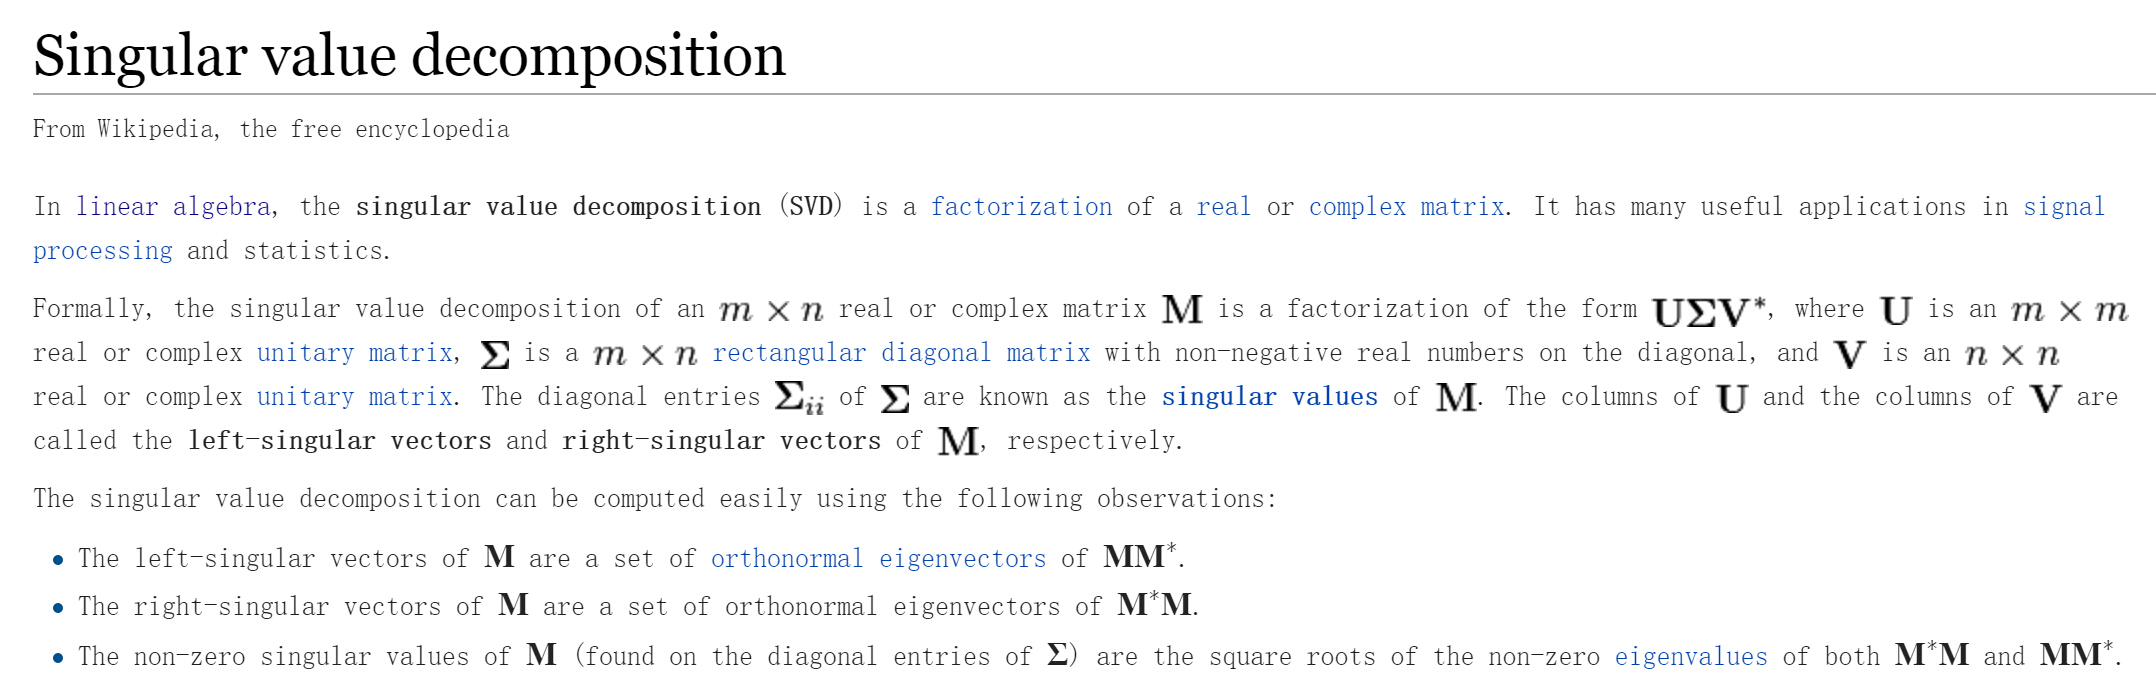
\includegraphics[width=1\textwidth]{1}
	\end{figure}
	
	\subsection{Principal Component Analysis}
	Principal component analysis (PCA) is a statistical procedure that uses an orthogonal transformation to convert a set of observations of possibly correlated variables into a set of values of linearly uncorrelated variables called principal components. The number of principal components is less than or equal to the number of original variables. This transformation is defined in such a way that the first principal component has the largest possible variance (that is, accounts for as much of the variability in the data as possible), and each succeeding component in turn has the highest variance possible under the constraint that it is orthogonal to the preceding components. The resulting vectors are an uncorrelated orthogonal basis set. The principal components are orthogonal because they are the eigenvectors of the covariance matrix, which is symmetric. PCA is sensitive to the relative scaling of the original variables.
	\subsection{The covariance matrix}
	An easy way to identify redundant data is by considering the covariance between data sets. Recall
	from our early chapters on probability and statistics that the covariance measures the statistical
	dependence/independence between two variables. Obviously, strongly statistically dependent
	variables can be considered as redundant observations of the system.
\subsection{Gabor}
The Gábor transform, also known as the short-time Fourier transform (STFT),is then defined as the following:
\begin{equation}
 \label{Gabor Transform}
 \hat{G}[f](t,w) = \tilde{f}_{g}(t,\omega) = \int_{-\infty}^{\infty} f(\tau) \bar{g}(\tau - t)\exp(-i\omega\tau)  d\tau
\end{equation}
where the bar denotes the complex conjugate of the function. Thus the function $g(\tau − t)$ acts as a time filter for localizing the signal over a specific window of time. The integration over the parameter $\tau$ slides the time-filtering window down the entire signal in order to pick out the frequency information at each instant of time. \\

More theory of Gabor on page322, 13.4 Time-Frequency Analysis: Windowed Fourier Transform.\\
Book:[J. Nathan Kutz] Data-Driven Modeling and Scientific Computation: Methods for Complex Systems and Big Data.









\section{Algorithm Implementation and Development}
For all music loaded in matlab, reduce the sampling rate by 100, substract mean and divide by variance to make them on same scale.
Then select time slide to do gabor transform to obtain the spectrum of each piece of music, just as HW2.
Obtaining the spectrums of the musics, put them in a matrix and do svd, obtain u,s,v and do cluster and classification on the v component. Using Gaussian mixed model and naive bayes to do the classification of the new genre of the musics.


\section{Computational Results}
\subsection{Test One}
I imported 3 type of music, rock by Guns N roses, pop by Jay chou and classical music by Dmitri Shostakovich, for which I select 3 different songs. \\
Guns n roses: Welcome to the jungle, Nightrain, Paradise city.\\
Jay chou: qing hua ci, ju hua tai, fa ru xue.\\
Dmitri Shostakovich: Waltz No.2, Romance, Piano Concerto No.2:II.Andante\\
For each song, chop it by 5 seconds, apply gabor transform to get the spectrum and repeat the steps for each song, I obtain a matrix filled with spectrums of 9 songs. By doing svd and I got the energy of the system, as shown in figure 2.\\
It's clear to see there is a dominant mode that the property is shared by 9 songs, so the emphasis is on the second, third and fourth mode.\\
By chosing the coresponding columns and rows of the v matrix, the dot plot is shown in figure 3. However it looks like there's only one cluster, and I zoomed in finding out that there are 3 clusters, as shown in figure 3 and 4.\\
Followed by the cross validation process, as shown in figure 5 and 6.
It's clear to see that the NaiverBayes does a better job, for the label should be an increased order as shown in figure 6. 
\begin{figure}[h]
	\centering
	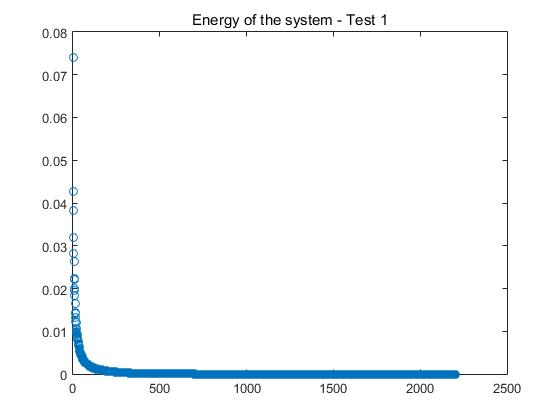
\includegraphics[width=3.0in]{p1}
	\caption{The energy of the system - Test one}
	
\end{figure}
\begin{figure}[h]
	\centering
	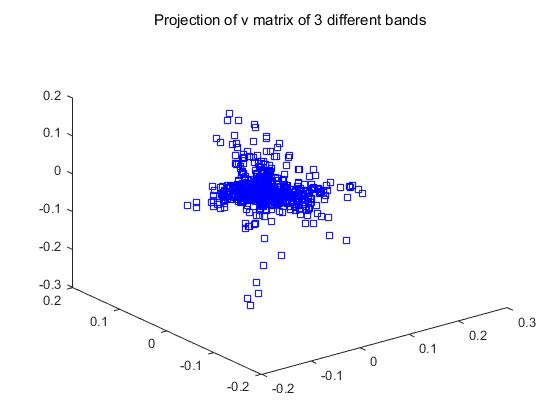
\includegraphics[width=5.0in]{p3}
	\caption{scatter of projection of v matrix - Test one}
	
\end{figure}
\begin{figure}[h]
	\centering
	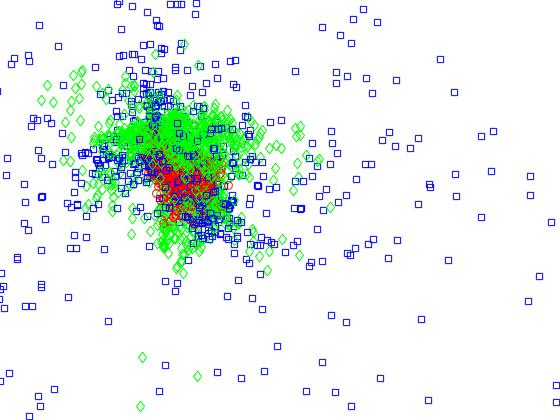
\includegraphics[width=3.0in]{p2}
	\caption{zoom in version of the figure 3}
	
\end{figure}
\begin{figure}[h]
	\centering
	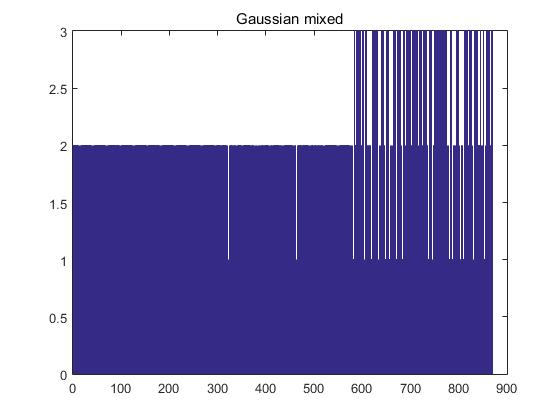
\includegraphics[width=3.0in]{p5}
	\caption{predictor: Gaussian mix - Test one}
	
\end{figure}

\begin{figure}[h]
	\centering
	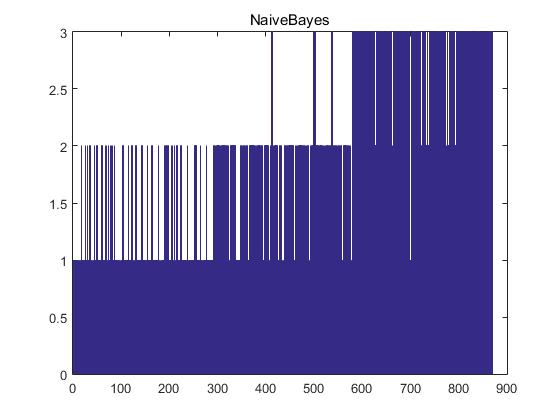
\includegraphics[width=3.0in]{p4}
	\caption{predictor: NaiveBayes - Test one}
	
\end{figure}

\subsection{Test Two}
In this section I focus on the bands that's all rock and Guns n roses, Alice in Chain, and Nirvana are chosen. \\
Guns n roses: Welcome to the jungle, Nightrain, Paradise city.\\
Alice in Chains: Don't follow, Would, Man in the box.\\
Nirvana: Smells Like Teen Spirit, Lithium,You Know You're Right\\
Redo the process again, instead change the 9 songs in the song list, we have the following:\\
figure 7 shows the energy of the system and a dominant mode. Figure 8 shows the cluster of 3 rock band. Figure 9 shows the gaussian fix model but it's not worked so well. And the Figure 10 shows the NaiveBayes, it works pretty well. But compared to the test one, it's hard to make accurate prediction in this case.
\begin{figure}[h]
	\centering
	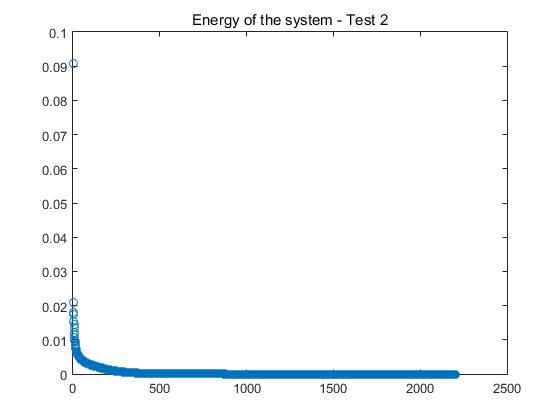
\includegraphics[width=3.0in]{p6}
	\caption{Energy of the System - Test two}
\end{figure}

\begin{figure}[h]
	\centering
	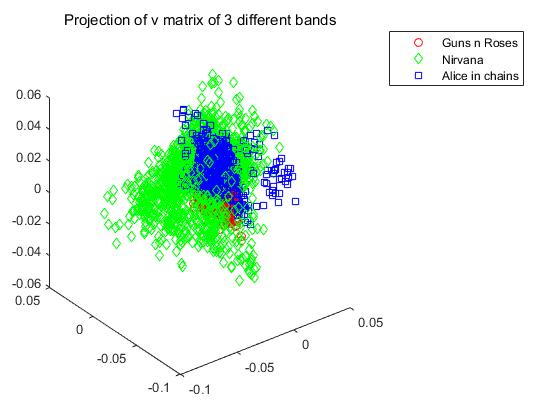
\includegraphics[width=5.0in]{p7}
	\caption{scatter of projection of v matrix - Test two}
\end{figure}

\begin{figure}[h]
	\centering
	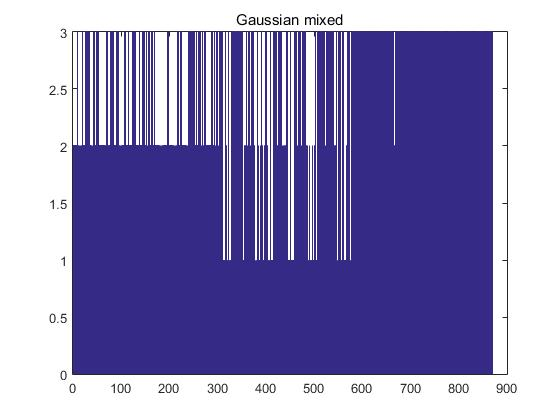
\includegraphics[width=5.0in]{p8}
	\caption{Gaussian mix - Test two}
\end{figure}
\begin{figure}[h]
	\centering
	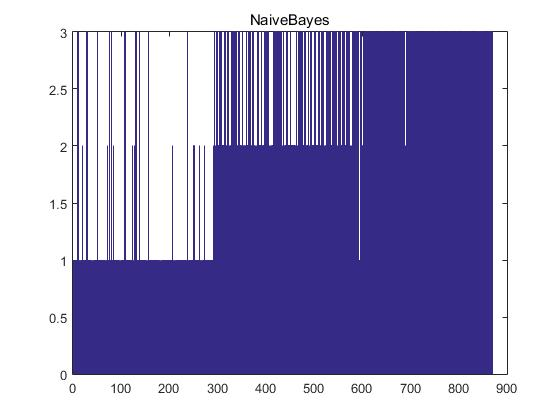
\includegraphics[width=5.0in]{p9}
	\caption{Naive Bayes - Test two}
\end{figure}

\subsection{Test Three}
In this case I chose 9 bands, 3 of a genre, rock, pop and classic.
Repeating the process above and get the following, as shown in figure 11, 12, 13 ,14.\\
It's harder to figure out the genre for the bands have their own characteristic so that the prediction cannot be easily made right.
\begin{figure}[h]
	\centering
	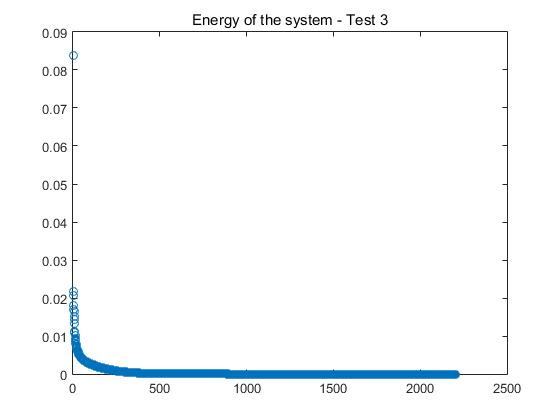
\includegraphics[width=3.0in]{p12}
	\caption{Energy of the System - Test three}
\end{figure}

\begin{figure}[h]
	\centering
	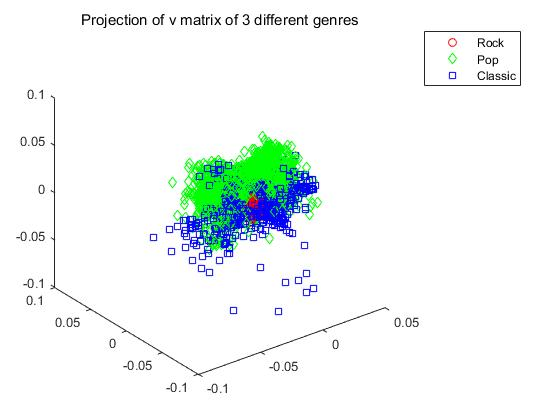
\includegraphics[width=5.0in]{p13}
	\caption{scatter of projection of v matrix - Test three}
\end{figure}

\begin{figure}[h]
	\centering
	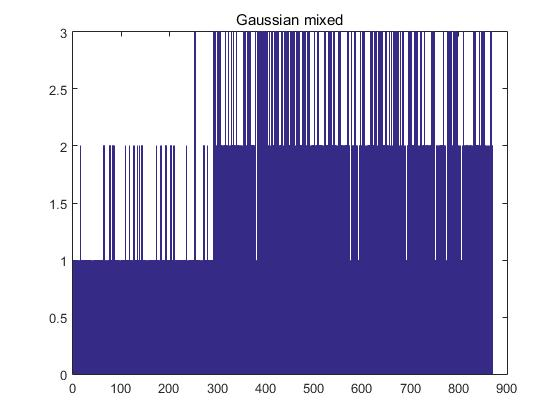
\includegraphics[width=5.0in]{p15}
	\caption{Gaussian mix - Test three}
\end{figure}
\begin{figure}[h]
	\centering
	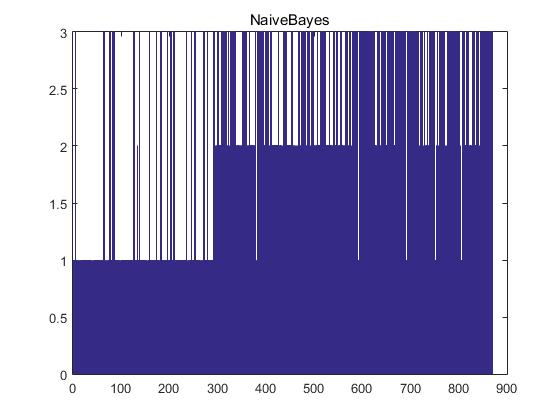
\includegraphics[width=5.0in]{p14}
	\caption{Naive Bayes - Test three}
\end{figure}

\section{Conclusion}
The analysis provides a view of deal with data, but it works depends on the selection of data.\
From test one and test two it shows that the NaiveBayes works pretty well in this course of machine learning and finding clusters, which provides a good way to make prediction of new data come in.






\appendix
\section{}
\subsection{linspace}
y = linspace(x1,x2,n) generates n points. The spacing between the points is (x2-x1)/(n-1).\\
In the code we have \\
$x2=linspace(-L,L,n+1);$\\
for FFT on a periodic boundary so the first point is the same as the last one. So we take n+1 mode and only pick the first n element.

\subsection{fft,fftshift,fftn}
fft,fft2,fftn transform the signal in 1D,2D and nD in to frequency domain with same dimension. When we do the tranformation, we must rescale the wavenumbers by $2*pi/L$ since the FFT assumes 2*pi periodic signals, where L is the spatial domain.

\subsection{meshgrid}
[X,Y,Z] = meshgrid(x,y,z) produces three-dimensional coordinate arrays. Make Matlab know your x, y ,z are perpendicular to each other.

\subsection{zeros, ones}
A = zeros(n,n,n) or ones(n,n,n) create a matrix with all zero and one entries with desired dimension

\subsection{reshape}
A = reshape(B,n,n) reshape a matrix with desired columns and rows

\subsection{max}
[m,I] = max(A);
A is a one dimensional matrix, m is the max number in the matrix and I is the index of m in A

\subsection{ind2sub}
The ind2sub command determines the equivalent subscript values corresponding to a single index into an array.

\subsection{classify}
class = classify(sample,training,group) classifies each row of the data in sample into one of the groups in training. sample and training must be matrices with the same number of columns. group is a grouping variable for training. Its unique values define groups; each element defines the group to which the corresponding row of training belongs. group can be a categorical variable, a numeric vector, a string array, or a cell array of strings. training and group must have the same number of rows. classify treats NaNs or empty strings in group as missing values, and ignores the corresponding rows of training. The output class indicates the group to which each row of sample has been assigned, and is of the same type as group.

\subsection{fitNaiveBayes}
NBModel = fitNaiveBayes(X,Y) returns a naive Bayes classifier NBModel, trained by predictors X and class labels Y for K-level classification.\\
Predict labels for new data by passing the data and NBModel to predict.


\begin{lstlisting}
clear all; close all; clc;
genre = cell(1,9);
genre{1,1} = 'GNRWJ.mp3';
genre{1,2} = 'GNRNT.mp3';
genre{1,3} = 'GNRPC.mp3';
% genre{1,4} = 'Jay Chou QHC.mp3';
% genre{1,5} = 'Jay Chou JHT.mp3';
% genre{1,6} = 'Jay Chou FRX.mp3';
genre{1,4} = 'NV_SS.mp3';
genre{1,5} = 'NV_UK.mp3';
genre{1,6} = 'NV_LI.mp3';
% genre{1,7} = 'DS-AND.mp3';
% genre{1,8} = 'DS-RO.mp3';
% genre{1,9} = 'DS-WN.mp3';
genre{1,7} = 'AIC MB.mp3';
genre{1,8} = 'AIC DF.mp3';
genre{1,9} = 'AIC W.mp3';
% 5 second
tr = 5;
songSpec = [];
for j = 1:9
currentSong = audioread(genre{1,j});
currentSong = currentSong(:,1);
%change sampling rate to pick 5-second clips and rescale
currentSong = decimate(currentSong,100);
currentSong = (currentSong - mean(currentSong))/var(currentSong);
% 5 second take 2205 position in the song, start at 10000 position of
% the song
clips = 30;
position = 10000;
L = 5; % 5 second of clips
tslide =  0: 0.25 : 5; 
width = 6;
allClipSpec = [];
for k = 1:30
currentClip = currentSong(position + 1:position + 2205,1);
position = position + 2205;
clipSpec = [];
for p = 1 : length(tslide)
% Gaussian filter
% time span
Fs = length(currentClip)/L;
t = (1:length(currentClip))/Fs;
g = exp(-width*(t - tslide(p)).^2);
% filter it out
currentClipf = g.*currentClip';

% Important !! fourier transform, the frequency content after the filter
currentClipft = abs(ifftshift(fft(currentClipf)));
clipSpec = [clipSpec currentClipft'];
end
allClipSpec = [allClipSpec clipSpec];
end
songSpec = [songSpec allClipSpec];
end
[u,s,v] = svd(songSpec,'econ');
sig = diag(s);
energy = sig/sum(sig);
figure(1)
plot(energy,'o');
title('Energy of the system - Test 2')
% figure(2)
% plot3(v(1:630,2),v(1:630,3),v(1:630,4),'rs');hold on;
% plot3(v(631:1260,2),v(631:1260,3),v(631:1260,4),'rd');hold on;
% plot3(v(1261:1890,2),v(1261:1890,3),v(1261:1890,4),'ro');hold on;
% plot3(v(1891:2520,2),v(1891:2520,3),v(1891:2520,4),'bo');hold on;
% plot3(v(2521:3150,2),v(2521:3150,3),v(2521:3150,4),'bs');hold on;
% plot3(v(3151:3780,2),v(3151:3780,3),v(3151:3780,4),'bd');hold on;
% plot3(v(3781:4410,2),v(3781:4410,3),v(3781:4410,4),'md');hold on;
% plot3(v(4411:5040,2),v(4411:5040,3),v(4411:5040,4),'mo');hold on;
% plot3(v(5041:5670,2),v(5041:5670,3),v(5041:5670,4),'ms');hold on;
figure(2)
plot3(v(1:1890,2),v(1:1890,3),v(1:1890,4),'ro');hold on;
plot3(v(1891:3780,2),v(1891:3780,3),v(1891:3780,4),'gd');hold on;
plot3(v(3781:5670,2),v(3781:5670,3),v(3781:5670,4),'bs');hold on;
title('Projection of v matrix of 3 different bands');
legend('Guns n Roses','Nirvana','Alice in chains')
% 
q1=randperm(1890);
q2=randperm(1890);
q3=randperm(1890);
rock = v(1:1890,2:4);
pop = v(1891:3780,2:4);
classic = v(3781:end,2:4);
xtrain=[rock(q1(1:1600),:);pop(q2(1:1600),:);classic(q3(1:1600),:)];
ctrain=[ones(1600,1);2*ones(1600,1);3*ones(1600,1)];
xtest=[rock(q1(1601:end),:);pop(q2(1601:end),:);classic(q3(1601:end),:)];



nb=fitNaiveBayes(xtrain,ctrain);
pre1=nb.predict(xtest);

gm = fitgmdist(xtrain,3);
pre2 = cluster(gm,xtest);


figure(3)
bar(pre1)
title('NaiveBayes')

figure(4)
bar(pre2)
title('Gaussian mixed')

% figure(4)
% plot3(v(1:630,2),v(1:630,3),v(1:630,4),'bs');hold on;
% plot3(v(631:1260,2),v(631:1260,3),v(631:1260,4),'rs');hold on;
% plot3(v(1261:1890,2),v(1261:1890,3),v(1261:1890,4),'gs');hold on;





\end{lstlisting}
\end{document}